\documentclass[12pt]{article}

\usepackage[charter]{mathdesign}
\usepackage[bookmarks,bookmarksopen]{hyperref}
\usepackage{bm}
\usepackage{graphicx}

\begin{document}
\section{Fixed Functions in Graphic Pipeline}
    \subsection{Rasterization}
        Addition Fomulars:
        \[ \begin{array}{c}
            \cos{ \left( x+y \right) }=\cos{x}\cos{y}-\sin{x}\sin{y} \\
            \sin{ \left( x+y \right) }=\sin{x}\cos{y}+\cos{x}\sin{y}
        \end{array} \]
        2D rotate matrix:
        \[ \left[ \begin{array}{rr}
            \cos{\alpha} & -\sin{\alpha} \\
            \sin{\alpha} & \cos{\alpha}
        \end{array} \right] \]
        2D matrix to rotate a vector 90 degress counter-clockwise:
        \[ \left[ \begin{array}{rr}
            0 & 0\\
            -1 & 0
        \end{array} \right] \]
        To judge vector v1 is pointing to the right side of vector v0:
        \[
        \left(
            \left[ \begin{array}{rr} 0 & 0\\ -1 & 0 \end{array} \right]
            \overrightarrow{v_0}
        \right)
        \cdot \overrightarrow{v_1} > 0
        \]
        In OpenGL, default visiable triangles are counter-clockwise, thus left side of 
        three edges form the triangle aera.
    \subsection{Coordinate System Transform}
        Describe (u,v,w) space axis in (x,y,z) space:
        \begin{eqnarray*}
            \left[ \begin{array}{ccc} \overrightarrow{u} & \overrightarrow{v} & \overrightarrow{w} \end{array} \right] &
            = &
            \left[ \begin{array}{ccc} \overrightarrow{x} & \overrightarrow{y} & \overrightarrow{z} \end{array} \right]
            \times
            \left[ \begin{array}{ccc}
                x_u & x_v & x_w \\
                y_u & y_v & y_w \\
                z_u & z_v & z_w
            \end{array} \right] \\
            & = &
            \left[ \begin{array}{ccc} \overrightarrow{x} & \overrightarrow{y} & \overrightarrow{z} \end{array} \right]
            \times
            \textbf{P}
        \end{eqnarray*}
        \textbf{P} converts a vector from (u,v,w) space to (x,y,z) space; Inv(\textbf{P})
        converts a vector from (x,y,z) space to (u,v,w) space:
        \begin{eqnarray*}
            \left[ \begin{array}{c} u_0 \\ v_0 \\ w_0 \end{array} \right] &
            = &
            \left[ \begin{array}{ccc}
                \overrightarrow{u} & \overrightarrow{v} & \overrightarrow{w}
            \end{array} \right]
            \times
            \left[ \begin{array}{c} u_0 \\ v_0 \\ w_0 \end{array} \right] \\
            & = &
            \left[ \begin{array}{ccc}
            \overrightarrow{x} & \overrightarrow{y} & \overrightarrow{z}
            \end{array} \right]
            \times
            \textbf{P}
            \times
            \left[ \begin{array}{c} u_0 \\ v_0 \\ w_0 \end{array} \right] \\
            & = &
            \left[ \begin{array}{ccc}
            \overrightarrow{x} & \overrightarrow{y} & \overrightarrow{z}
            \end{array} \right]
            \times
            \left(
                \textbf{P}
                \times
                \left[ \begin{array}{c} u_0 \\ v_0 \\ w_0 \end{array} \right]
            \right)
        \end{eqnarray*}
        For points transformation:
        \[
            \left[ \begin{array}{cc}
                \textbf{P} & \begin{array}{c} u_{root} \\ v_{root} \\ w_{root} \end{array} \\
                \begin{array}{ccc} 0 & 0 & 0 \end{array} & 1
            \end{array} \right]
            \times
            \left[ \begin{array}{cc}
                \bm{P^{-1}} &
                -\bm{P^{-1}} \times
                \left[ \begin{array}{c}
                    u_{root} \\ v_{root} \\ w_{root}
                \end{array} \right] \\
                \begin{array}{ccc} 0 & 0 & 0 \end{array} &
                1
            \end{array} \right]
            =
            \left[ \begin{array}{cccc}
                1 & 0 & 0 & 0 \\
                0 & 1 & 0 & 0 \\
                0 & 0 & 1 & 0 \\
                0 & 0 & 0 & 1
            \end{array} \right]
        \]
    \subsection{Tangent Space}
        Triangle ABC in (x,y,z) space and (t,b,n) space:
        \[
            \left[ \begin{array}{ccc}
            x_a & x_b & x_c \\
            y_a & y_b & y_c \\
            z_a & z_b & z_c
            \end{array} \right]
            \left[ \begin{array}{ccc}
            u_a & u_b & u_c \\
            v_a & v_b & v_c \\
            0   & 0   & 0
            \end{array} \right]
        \]
        For 2 edges of the triangle:
        \begin{eqnarray*}
            \left[ \overrightarrow{x}, \overrightarrow{y}, \overrightarrow{z} \right]       
            \times
            \left[ \begin{array}{cc}
                E1_x & E2_x \\
                E1_y & E2_y \\
                E1_z & E2_z
            \end{array} \right]
            & = &
            \left[ \overrightarrow{t}, \overrightarrow{b}, \overrightarrow{n} \right]       
            \times
            \left[ \begin{array}{cc}
                E1_u & E2_u \\
                E1_v & E2_v \\
                0    & 0
            \end{array} \right] \\
            & = &
            \left[ \overrightarrow{t}, \overrightarrow{b} \right]       
            \times
            \left[ \begin{array}{cc}
                E1_u & E2_u \\
                E1_v & E2_v
            \end{array} \right]
        \end{eqnarray*}
        Then:
        \begin{eqnarray*}
            \left[ \overrightarrow{t}, \overrightarrow{b} \right]       
            & = &
            \left[ \overrightarrow{x}, \overrightarrow{y}, \overrightarrow{z} \right]       
            \times
            \left[ \begin{array}{cc}
                E1_x & E2_x \\
                E1_y & E2_y \\
                E1_z & E2_z
            \end{array} \right]
            \times
            \left[ \begin{array}{cc}
                E1_u & E2_u \\
                E1_v & E2_v
            \end{array} \right]^{-1} \\
            & = &
            \left[ \overrightarrow{x}, \overrightarrow{y}, \overrightarrow{z} \right]       
            \times
            \left(
                \left[ \begin{array}{cc}
                    E1_x & E2_x \\
                    E1_y & E2_y \\
                    E1_z & E2_z
                \end{array} \right]
                \times
                \left[ \begin{array}{cc}
                    E1_u & E2_u \\
                    E1_v & E2_v
                \end{array} \right]^{-1}
            \right) \\
            & = &
            \left[ \overrightarrow{x}, \overrightarrow{y}, \overrightarrow{z} \right]       
            \times
            \left(
                \left[ \begin{array}{cc}
                    E1_x & E2_x \\
                    E1_y & E2_y \\
                    E1_z & E2_z
                \end{array} \right]
                \times
                \frac{1}{E1_uE2_v-E1_vE2_u}
                \left[ \begin{array}{cc}
                     E2_v & -E2_u \\
                    -E1_v &  E1_u
                \end{array} \right]^{-1}
            \right) \\
            & = &
            \left[ \overrightarrow{x}, \overrightarrow{y}, \overrightarrow{z} \right]       
            \times
            \left(
                \frac{1}{E1_uE2_v-E1_vE2_u}
                \left[ \begin{array}{cc}
                    E1_x & E2_x \\
                    E1_y & E2_y \\
                    E1_z & E2_z
                \end{array} \right]
                \times
                \left[ \begin{array}{cc}
                     E2_v & -E2_u \\
                    -E1_v &  E1_u
                \end{array} \right]^{-1}
            \right)
        \end{eqnarray*}

    \subsection{Perspective Projection}
    In perspective projection, r,n,f\(\left[\alpha,\beta\right]\) defines a frustum:
    \begin{itemize}
        \item f: z of far plane
        \item n: z of near plane
        \item r: ratio of width to height of view wnidow
        \item d: z of view window
        \item \(\alpha\) : view angle in the y axis direction
        \item \(\beta\) : view angle in the x axis direction
    \end{itemize}
    In the y axis direction:
    \begin{center}
        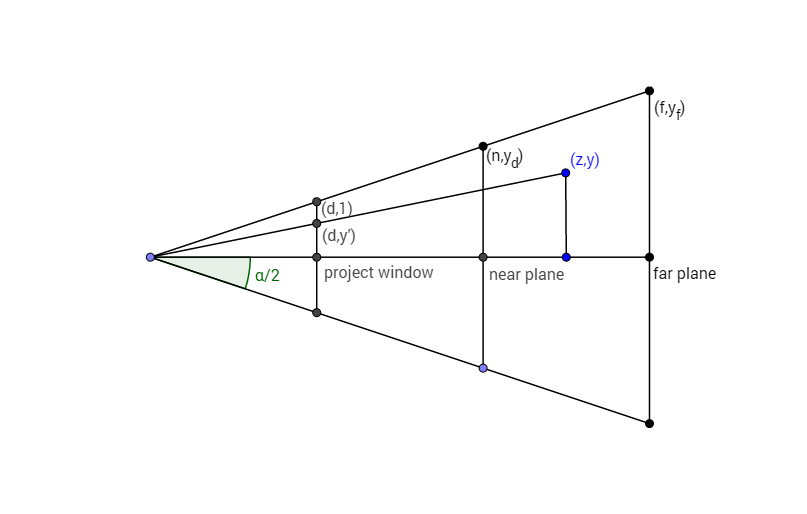
\includegraphics[height=25em]{geogebra/project_y.png}
    \end{center}
    \[
        y'=y\frac{d}{z}=\frac{y}{z\tan{\frac{\alpha}{2}}}
    \]
    And in the x axis direction:
    \begin{center}
        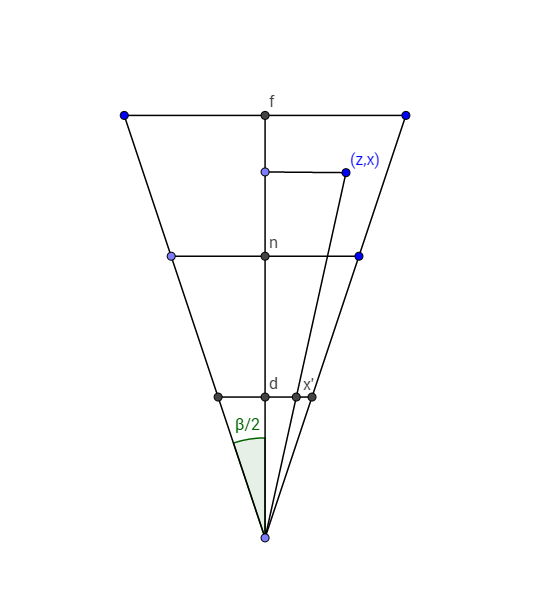
\includegraphics[height=25em]{geogebra/project_x.png}
    \end{center}
    \[
        x'=x\frac{d}{z}=\frac{x}{z\bullet r\tan{\frac{\alpha}{2}}}
    \]
    Put everything together:
    \[
        \left[ \begin{array}{cccc}
            \frac{1}{r\tan{\frac{\alpha}{2}}} & & & \\
            & \frac{1}{\tan{\frac{\alpha}{2}}} & & \\
            & & A & B \\
            & & 1 & 0
        \end{array} \right]
        \left[ \begin{array}{c}
            x \\
            y \\
            z \\
            1
        \end{array} \right]
        =
        \left[ \begin{array}{c}
            \frac{x}{r\tan{\frac{\alpha}{2}}} \\
            \frac{y}{\tan{\frac{\alpha}{2}}} \\
            A\bullet z+B \\
            z
        \end{array} \right]
        \to
        \left[ \begin{array}{c}
            \frac{x}{r\bullet z\tan{\frac{\alpha}{2}}} \\
            \frac{y}{z\tan{\frac{\alpha}{2}}} \\
            A+\frac{B}{z} \\
            1
        \end{array} \right]
    \]
    To make \(A+\frac{B}{z}\) 0 at near plane and -1 at far plane:
    \begin{itemize}
        \item \(A=\frac{-f}{f-n}\)
        \item \(B=\frac{nf}{f-n}\)
    \end{itemize}
    
\section{Linear Algebra}
    \subsection{Cross Product}
    Cross product definition differs in right-hand coordinate system and left-hand
    coordinate system ensuring that:
    \[ \begin{array}{c}
        \overrightarrow{x} \times \overrightarrow{y} = \overrightarrow{z} \\
        \overrightarrow{y} \times \overrightarrow{z} = \overrightarrow{x} \\
        \overrightarrow{z} \times \overrightarrow{x} = \overrightarrow{y}
    \end{array} \]
    From this, it can be inferred that:
    \begin{eqnarray*}
        \left[ \begin{array}{c}
            a_1 \\ a_2 \\ a_3
        \end{array} \right]
        \times
        \left[ \begin{array}{c}
            b_1 \\ b_2 \\ b_3
        \end{array} \right] &
        = &
        \left(
            a_1\overrightarrow{x} + a_2\overrightarrow{y} + a_3\overrightarrow{z}
        \right)
        \times
        \left(
            a_1\overrightarrow{x} + a_2\overrightarrow{y} + a_3\overrightarrow{z}
        \right) \\
        & = &
        \left| \begin{array}{ccc}
            \overrightarrow{x} & \overrightarrow{y} & \overrightarrow{z} \\
            a_1 & a_2 & a_3 \\
            b_1 & b_2 & b_3
        \end{array} \right|
    \end{eqnarray*}
\end{document}